% ======================================================
% Compile: xelatex 6state_curvature_hd.tex
% Path:    reference/eq17_analysis/derivation/6state_curvature_hd.tex
% Purpose: Full-detail derivation of the 6-state curvature-Taylor eq17 controller
%          + closed-loop EKF, following the section-by-section flow of the baseline
%          RevisedConrol_Vpersonal.pdf (transcribed in 6state_derivation_xd.tex),
%          with three modifications:
%            (1) disturbance estimation dropped (delta_h_D stays in the plant,
%                uncompensated -- EKF models it as 0), as in 5state_derivation.tex;
%            (2) the gain is a Taylor expansion about the desired height
%                a_h = a_h(h_d) - a'_hd * delta_h  (merges 4state_taylor_gain);
%            (3) a'_hd evolves via the curvature state:
%                a'_hd[k+1]       = a'_hd[k] + Dh_d[k] * delta_a'_hd[k],
%                delta_a'_hd[k+1] = delta_a'_hd[k].
%          h-notation (a_h, h_d, delta_h, F_dh, eps_h, e_ah, a'_hd, delta_a'_hd)
%          per the user's manuscript. Scope: ends at the boxed 6x6 F_e (Q left as
%          the symbol q[k], as in the baseline).
%          State x = [ dh1, dh2, dh3, a_h, a'_hd, delta_a'_hd ].
% Style mirrors 5state_derivation / 6state_derivation_xd (monochrome, \fbox on key
% results, run-in bold-underline \hd headings).
% ---- BUILD STATUS: Stage S6 (sections 1-12; complete to the boxed 6x6 F_e). RESTRUCTURED as
%      True state equation (EXACT curve, all Taylor orders) -> Estimator (our truncated model:
%      a_h 1st-order, a'_hd swept, delta_a'_hd FROZEN, unchanged since it is all we can implement
%      with c(h) unknown) -> Error dynamics = True - Estimator. The model mismatch then surfaces:
%      q3=-eps_h, q4=a'_hd*eps_h (thermal, in both); q6 = a'''_hd*Dh (the TRUE 3rd-order curvature
%      sweep that the frozen delta_a'_hd estimator misses) reappears with a clear source and is
%      trajectory-driven (propto Dh, zero on a hold) -> Q66 = a'''^2 Dh^2, Q55=0. 2nd-order
%      residuals (1/2 a'' dh^2, 1/2 a''' Dh^2) dropped. Curvature bias in a_hm noted (R2 deferred).
%      Q66 CLOSURE: q6 keeps a''' symbolically (true term), but Q66 avoids the a''' -> a'''' ->
%      ... derivative regress by the top-state closure a''' ~ delta_a'_hd/R => Q66 ~ (delta_a'_hd*Dh/R)^2
%      (trajectory-gated, no higher derivative needed). L*r dropped. Full Q/R + near-wall cap deferred. ----
% ======================================================
\documentclass[11pt,a4paper,fontset=none]{ctexart}

\usepackage[fleqn]{amsmath}
\usepackage{amssymb,bm}
\usepackage{empheq}
\setlength{\mathindent}{0pt}
\usepackage{geometry}
\geometry{margin=2.0cm}
\usepackage{enumitem}
\usepackage{array,booktabs}
\usepackage{titlesec}
\usepackage{graphicx}

\setlength{\parindent}{0pt}
\setlength{\parskip}{0.75em}
\linespread{1.08}
\setlength{\abovedisplayskip}{9pt}
\setlength{\belowdisplayskip}{9pt}
\setlength{\abovedisplayshortskip}{5pt}
\setlength{\belowdisplayshortskip}{5pt}

% --- Shortcuts (h-notation) ---
\newcommand{\lc}{\lambda_c}
\newcommand{\Dh}{\Delta h_d}
\newcommand{\DHd}{\Delta H_d}
\newcommand{\Fdh}{F_{dh}}
\newcommand{\FdhH}{F_{dh}^{\Delta H}}
\newcommand{\ap}{a'_{hd}}
\newcommand{\aph}{\hat a'_{hd}}
\newcommand{\dap}{\delta a'_{hd}}
\newcommand{\daph}{\delta \hat a'_{hd}}
\newcommand{\tap}{a'''_{hd}}
\newcommand{\eah}{e_{a_h}}
\newcommand{\eap}{e_{a'_{hd}}}
\newcommand{\edap}{e_{\delta a'_{hd}}}
\newcommand{\hd}[1]{\par\medskip\noindent\underline{\textbf{#1}}\par\nobreak\vspace{0.2ex}}

\begin{document}

\hd{Equation of motion}
\[ h[k+1] = h[k] + a_h[k]\{f_{dh}[k] + f_T[k]\} + \delta h_D[k], \]

\hd{Motion error}
\[ \delta h[k+1] = \delta h[k] + \Dh[k] - a_h[k]\{f_{dh}[k] + f_T[k]\} - \delta h_D[k], \]

$\delta h[k] = h_d[k] - h[k]$, $h_d[k]$ is the desired motion trajectory, $\delta h_D[k]$ is the motion error caused by the disturbance, and $\Dh[k] = h_d[k+1] - h_d[k]$ is the desired motion step size.

\hd{Measurement} (\textit{d}-step delay)
\[ \delta h_m[k] = \delta h[k-d] + n_h[k], \]

\noindent\underline{\textbf{Control objective}}: $\;\delta h[k+1] = \lc \cdot \delta h[k];\quad 0 \le \lc < 1$

\medskip
\textit{Ideal control effort (no measurement delay)}:
\[ \bar f_{dh}[k] = a_h^{-1}[k]\{\Dh[k] + (1-\lc)\,\bm{\delta h[k]} - \delta h_D[k]\} \]

\textit{Motion error}:
\[ \delta h[k+1] = \delta h[k] + \Dh[k] - a_h[k]\{\bar f_{dh}[k] + f_T[k]\} - \delta h_D[k] = \lc \cdot \delta h[k] - a_h[k] f_T[k] \]

\textit{d-step measurement delay}:
\[ \bm{\delta h[k]} = \delta h[k-d] + \sum_{i=1}^{d}\Dh[k-i] - \sum_{i=1}^{d} a_h[k-i]\{f_{dh}[k-i] + f_T[k-i]\} - \sum_{i=1}^{d}\delta h_D[k-i] \]

\textit{Ideal control effort (with d-step measurement delay)}:
\[
\begin{aligned}
\bar{\bar f}_{dh}[k] = a_h^{-1}[k]\Big\{
& \underbrace{\Big[\Dh[k] + (1-\lc)\textstyle\sum_{i=1}^{d}\Dh[k-i]\Big]}_{\Delta h_d^{d}[k]}
+ (1-\lc)\Big[\delta h[k-d] - \textstyle\sum_{i=1}^{d} a_h[k-i] f_{dh}[k-i]\Big] \\
& - \underbrace{\Big[\delta h_D[k] + (1-\lc)\textstyle\sum_{i=1}^{d}\delta h_D[k-i]\Big]}_{\delta h_D^{d}[k]}
\Big\}
\end{aligned}
\]

\textit{Motion error}:
\[
\delta h[k+1] = \lc \cdot \delta h[k] - \underbrace{\Big\{ a_h[k] f_T[k] + (1-\lc)\textstyle\sum_{i=1}^{d} a_h[k-i] f_T[k-i] \Big\}}_{\delta h_T^{d}[k]}
\]

\hd{Implementable control effort} \;{\small ($\delta \hat h_D^{d}\!\equiv\!0$: disturbance not estimated)}
\begin{empheq}[box=\fbox]{equation*}
f_{dh}[k] = \hat a_h^{-1}[k]\Big\{ \Delta h_d^{d}[k] + (1-\lc)\Big[\delta h_m[k] - \textstyle\sum_{i=1}^{d}\hat a_h[k-i] f_{dh}[k-i]\Big] \Big\}
\end{empheq}

\hd{Motion error}
\[ \delta h[k+1] = \lc \cdot \delta h[k] - a_h[k]\big[ f_{dh}[k] - \bar{\bar f}_{dh}[k] \big] - \delta h_T^{d}[k] \]

\[ a_h[k]\,\bar{\bar f}_{dh}[k] = \Delta h_d^{d}[k] + (1-\lc)\Big[\delta h[k-d] - \textstyle\sum_{i=1}^{d} a_h[k-i] f_{dh}[k-i]\Big] - \delta h_D^{d}[k] \]

\[
a_h[k]\, f_{dh}[k] = \big(1 + e_{a_h}[k]\,\hat a_h^{-1}[k]\big)\Big\{ \Delta h_d^{d}[k]
+ (1-\lc)\Big[\big(\delta h[k-d] + n_h[k]\big) - \textstyle\sum_{i=1}^{d}\hat a_h[k-i] f_{dh}[k-i]\Big] \Big\}
\]

\[
\begin{aligned}
a_h[k]\, f_{dh}[k] - a_h[k]\,\bar{\bar f}_{dh}[k] ={}& e_{a_h}[k]\, f_{dh}[k] + (1-\lc) n_h[k] \\
&+ (1-\lc)\textstyle\sum_{i=1}^{d}\big(a_h[k-i] - \hat a_h[k-i]\big) f_{dh}[k-i] + \delta h_D^{d}[k]
\end{aligned}
\]

\textit{Gain model} \;{\small (exact curve; definitions only)}:
\begin{empheq}[box=\fbox]{align*}
a_h[k] &= a_h(h_d[k]) - \ap[k]\,\delta h[k], & a_h(h_d[k{+}1]) &= a_h(h_d[k]) + \ap[k]\,\Dh[k], \\
\ap &:= \tfrac{d a_h}{d h}\Big|_{h_d}, \;\; \dap := \tfrac{d^2 a_h}{d h^2}\Big|_{h_d}, & \tap &:= \tfrac{d^3 a_h}{d h^3}\Big|_{h_d}.
\end{empheq}

\textit{Gain-error back-step}:
\[ a_h[k-i] - \hat a_h[k-i] \approx e_{a_h}[k] - \big(h_d[k]-h_d[k-i]\big)\, e_{\ap}[k] \]
\[
\begin{aligned}
a_h[k]\, f_{dh}[k] - a_h[k]\,\bar{\bar f}_{dh}[k] \approx{}&
e_{a_h}[k]\,\underbrace{\Big\{ f_{dh}[k] + (1-\lc)\textstyle\sum_{i=1}^{d} f_{dh}[k-i] \Big\}}_{\Fdh[k]} \\
&- e_{\ap}[k]\,\underbrace{\Big\{ (1-\lc)\textstyle\sum_{i=1}^{d} \big(h_d[k]-h_d[k-i]\big) f_{dh}[k-i] \Big\}}_{\FdhH[k]} \\
&+ \delta h_D^{d}[k] + (1-\lc) n_h[k]
\end{aligned}
\]

\begin{empheq}[box=\fbox]{align*}
\delta h[k+1] ={}& \lc \cdot \delta h[k] - \Fdh[k]\cdot e_{a_h}[k] + \FdhH[k]\cdot e_{\ap}[k] - \delta h_D^{d}[k] \\
&- \underbrace{\big\{ \delta h_T^{d}[k] + (1-\lc) n_h[k] \big\}}_{\varepsilon_h[k]}
\end{empheq}

\hd{True gain recursion} \;{\small (exact curve values swept to $h_d[k{+}1]$; $[\,\cdot\,]$ = residual the estimator drops)}
\[ a_h[k+1] = a_h(h_d[k+1]) - \ap[k+1]\,\delta h[k+1], \quad
   \ap[k+1] = a_h'(h_d[k+1]), \quad \dap[k+1] = a_h''(h_d[k+1]) \]
\begin{empheq}[box=\fbox]{align*}
a_h[k+1]  &= a_h + \ap\,\Dh + (1{-}\lc)\ap\,\delta h + \ap\,\Fdh\,\eah + \ap\,\varepsilon_h
           \;\big[\,+\tfrac12\dap\,\delta h[k{+}1]^2\,\big] \\
\ap[k+1]  &= \ap + \dap\,\Dh \;\big[\,+\tfrac12\tap\,\Dh^2\,\big] \\
\dap[k+1] &= \dap + \tap\,\Dh
\end{empheq}

\hd{True state equation} \;{\small ($\delta h_D^{d}\!\equiv\!0$; leading order)}
\[
\begin{aligned}
\delta h_1[k+1] &= \delta h_2[k] \\
\delta h_2[k+1] &= \delta h_3[k] \\
\delta h_3[k+1] &= \lc\,\delta h_3[k] - \Fdh[k]\,\eah[k] + \FdhH[k]\,\eap[k] - \varepsilon_h[k] \\
a_h[k+1] &= a_h[k] + \ap\,\Dh + (1{-}\lc)\ap\,\delta h_3 + \ap\,\Fdh\,\eah + \ap\,\varepsilon_h \\
\ap[k+1] &= \ap[k] + \dap[k]\,\Dh \\
\dap[k+1] &= \dap[k] + \tap[k]\,\Dh
\end{aligned}
\]

\hd{Output equation}
\[
\begin{cases}
y_1[k] = \delta h_m[k] = \delta h_1[k] + \underbrace{n_h[k]}_{r_1[k]} \\[2.0ex]
y_2[k] = \underbrace{a_h[k-d] + n_a[k]}_{a_{hm}[k]} \approx a_h[k] - \DHd[k]\,\ap[k] + \underbrace{n_a[k]}_{r_2[k]}, \quad \DHd[k] := h_d[k]-h_d[k-d]
\end{cases}
\]
\[ \mathbf{H} = \begin{bmatrix} 1 & 0 & 0 & 0 & 0 & 0 \\ 0 & 0 & 0 & 1 & -\DHd[k] & 0 \end{bmatrix}, \qquad \mathbf{y}[k] = \mathbf{H}\,\mathbf{x}[k] + \mathbf{r}[k] \]
{\small (the thermal-based $a_{hm}$ additionally carries a curvature bias $\tfrac12\dap\,\sigma_h^2$ from the thermal excursion $\sigma_h^2$; folded into $r_2$/$R_2$, deferred.)}

\hd{Estimator (model)} \;{\small (truncated: $\hat a_h$ 1st-order, $\aph$ swept, $\daph$ \emph{frozen} $\Rightarrow$ drops the true $\tap\Dh$)}
\[ e_{\delta h_1} = \delta h_1 - \delta \hat h_1, \quad
   \eah = a_h - \hat a_h, \quad
   \eap = \ap - \aph, \quad
   \edap = \dap - \daph \]
\[ e_{y_1} = y_1 - \hat y_1 = \delta h_m - \delta \hat h_1 = e_{\delta h_1} + \underbrace{n_h}_{r_1} \]
\[ e_{y_2} = y_2 - \hat y_2 = a_{hm} - \big(\hat a_h - \DHd\,\aph\big) = \eah - \DHd\,\eap + \underbrace{n_a}_{r_2} \]
\[
\begin{aligned}
\delta \hat h_1[k+1] &= \delta \hat h_2 + \ell_{11}\, e_{y_1} + \ell_{12}\, e_{y_2} \\
\delta \hat h_2[k+1] &= \delta \hat h_3 + \ell_{21}\, e_{y_1} + \ell_{22}\, e_{y_2} \\
\delta \hat h_3[k+1] &= \lc\, \delta \hat h_3 + \ell_{31}\, e_{y_1} + \ell_{32}\, e_{y_2} \\
\hat a_h[k+1] &= \hat a_h + \aph\,\Dh + (1{-}\lc)\aph\,\delta \hat h_3 + \ell_{41}\, e_{y_1} + \ell_{42}\, e_{y_2} \\
\aph[k+1] &= \aph + \daph\,\Dh + \ell_{51}\, e_{y_1} + \ell_{52}\, e_{y_2} \\
\daph[k+1] &= \daph + \ell_{61}\, e_{y_1} + \ell_{62}\, e_{y_2}
\end{aligned}
\]

\hd{Error dynamics} \;{\small (True $-$ Estimator)}
\[
\begin{aligned}
e_{\delta h_1}[k+1] &= e_{\delta h_2} - \ell_{11}\,e_{\delta h_1} - \ell_{12}\,\eah + \ell_{12}\,\DHd\,\eap \\
e_{\delta h_2}[k+1] &= e_{\delta h_3} - \ell_{21}\,e_{\delta h_1} - \ell_{22}\,\eah + \ell_{22}\,\DHd\,\eap \\
e_{\delta h_3}[k+1] &= \lc\,e_{\delta h_3} - \Fdh\,\eah + \FdhH\,\eap - \underbrace{\varepsilon_h}_{q_3} \\
&\quad - \ell_{31}\,e_{\delta h_1} - \ell_{32}\,\eah + \ell_{32}\,\DHd\,\eap \\
\eah[k+1] &= (1{+}\ap\Fdh)\,\eah + (1{-}\lc)\ap\,e_{\delta h_3} + \Dh\,\eap + \underbrace{\ap\,\varepsilon_h}_{q_4} \\
&\quad - \ell_{41}\,e_{\delta h_1} - \ell_{42}\,\eah + \ell_{42}\,\DHd\,\eap \\
\eap[k+1] &= \eap + \Dh\,\edap - \ell_{51}\,e_{\delta h_1} - \ell_{52}\,\eah + \ell_{52}\,\DHd\,\eap \\
\edap[k+1] &= \edap + \underbrace{\tap\,\Dh}_{q_6} - \ell_{61}\,e_{\delta h_1} - \ell_{62}\,\eah + \ell_{62}\,\DHd\,\eap
\end{aligned}
\]

\begin{empheq}[box=\fbox]{equation*}
\mathbf{F}_e[k] =
\begin{bmatrix}
0 & 1 & 0 & 0 & 0 & 0 \\
0 & 0 & 1 & 0 & 0 & 0 \\
0 & 0 & \lc & -\Fdh & \FdhH & 0 \\
0 & 0 & (1{-}\lc)\ap & 1{+}\ap\Fdh & \Dh & 0 \\
0 & 0 & 0 & 0 & 1 & \Dh \\
0 & 0 & 0 & 0 & 0 & 1
\end{bmatrix}
\end{empheq}
\[ \mathbf{e}[k+1] = \mathbf{F}_e[k]\,\mathbf{e}[k] - \mathbf{L}[k]\,\mathbf{H}\,\mathbf{e}[k] + \mathbf{q}[k] \]
{\small $\mathbf q = [\,0,0,q_3,q_4,0,q_6\,]^\top$: $q_3{=}-\varepsilon_h$, $q_4{=}\ap\varepsilon_h$ (thermal); $q_6{=}\tap\Dh$ (the true 3rd-order sweep the frozen $\daph$ misses). $Q_{33}{=}\sigma_\varepsilon^2$, $Q_{44}{=}{\ap}^2\sigma_\varepsilon^2$, $Q_{55}{=}0$.}

\vspace{-0.3em}
{\small \textbf{Closure for $Q_{66}$}: taking $Q_{66}{=}{\tap}^2\Dh^2$ needs $\tap$, whose own noise needs $a^{(4)},a^{(5)},\dots$ --- an unclosed derivative regress. Since $a^{(n)}{=}(a_{nom}/R^{n})D^{(n)}$, each derivative scales by $1/R$, so close the hierarchy at the top state via $\tap\!\sim\!\dap/R$:
$\;\boxed{\,Q_{66}\approx\big({\dap}\,\Dh/R\big)^2\,}$ --- uses only the estimated $\daph$ and known $R,\Dh$ (no $\tap$); trajectory-gated ($\propto\Dh^2$, zero on a hold) and self-scaling to the curvature.}

\newpage
\begin{center}
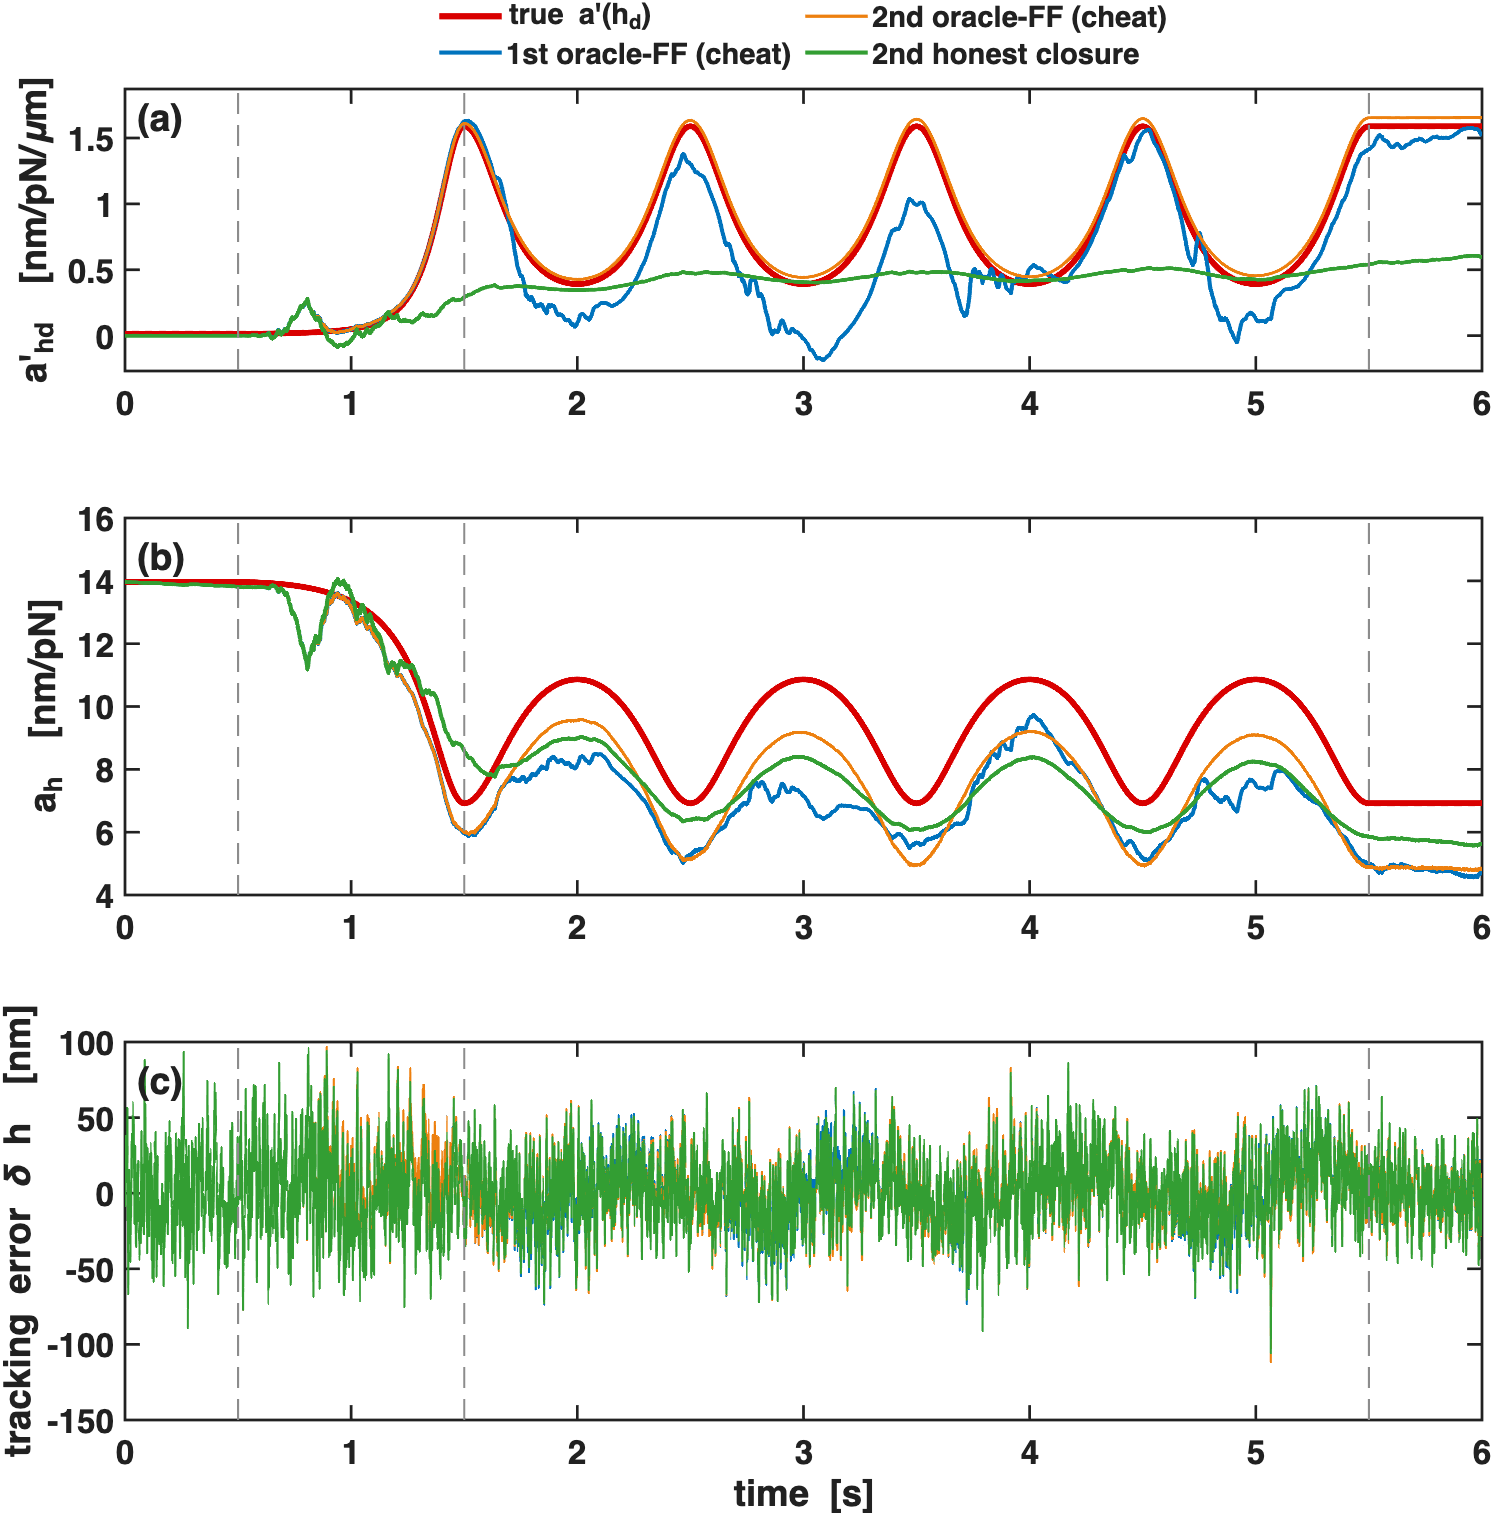
\includegraphics[width=\linewidth]{figures/aprime_hd_cheat_vs_honest.png}
\end{center}

\end{document}
